\documentclass{beamer}

\begin{document}
	\begin{frame}
	\frametitle{Introduction to Hypergraphs}

	Otherwise known as ``What I did last summer...''

	\end{frame}
	
	\begin{frame}	
	\frametitle{Review Basic Enumerable \& Indexable Types}
	\begin{center}
	\begin{itemize}
	\item Arrays\\
	\item Lists, Queues, Stacks
	\item Binary-Trees, N-way Trees
	\item Directed \& Undirected graphs
	\end{itemize}	
	\end{center}
	\end{frame}
	
	
	\begin{frame}	
	\frametitle{Nomenclature of hypernets and sets }
	\begin{center}
	The nomenclature surounding these this complex mathematical objects is varried, the first appearances assign the name ``hyper-graph'' as an extention on the graph-theory at the time (1960-80) ~ Citations are in the mail. \\
	\end{center}
\vspace{20 pt}
	\begin{center}
	Hyper-$net$, multigraph, multiple-edges,multiple-node-graph, intersection-graph, Clique graph, 3-sat microstructure complements, permutation set, power set, combination set, multi-sample-knapsack problem, all solutions to all problems from:\\
	\vspace{10 pt}
	 $O(c) \leq O(N) \leq O(N^c) \leq O(c^N) \leq O(N^N) \leq O(N^M)$ 
	\end{center}
	\end{frame}

	\begin{frame}	
	\frametitle{Applications of hypergraphs }
	\begin{itemize}
	\item Accuratly model the many body problem in physics.
	\item Model all reactions given a set of compounds.
	\item Model all phone calls in a telephony network.
	\item All cycles in a standard graph	
	\item Roughly corresponds to writing a struct or class in programming.
	\item Related to group theory in mathematics.
	\end{itemize}		
	\end{frame}	
	
	\begin{frame}	
	\frametitle{Dense vs fully connected graph vs hypernet}
	\begin{itemize}
	\item A dense graph has up to $N^2$ edges
	\item A fully connected graph has $N^2$ edges.
	\item A fully connected unrestricted hypergraph has $N^{\infty}$ edges.
	\item A hyper-edge contains a set of nodes that can repeat.
	\item A hyper-graph contains the set of all nodes.
	\item A hyper-net contains all possible solutions to the problem.
	\item Finding the correct ordering of nodes \& edges for the given hypergraph instance is equivelent to checking the `set of all answers' for the correct answer for your problem.
	\end{itemize}		
	\end{frame}
	
	\begin{frame}	
	\frametitle{Hypernet as a representation}
	\begin{itemize}
	\item As hypernets contain an infinite number of edges; thus no `real' instance can be created.
	\item A hypernet model can be built to access the infinite edges.
	\item A hypergraph is an instance that maps indexes to nodes and nodes to indexs.
	\item An odometer is an instance of an indexed set of numbers.
	\item A hyper-edge is an instance of an indexed set of nodes
	\item Odometers correspond $1:1$ with hyper-edges given a hypergraph.
	\item Elegant mechanicst: code reduces to a vector of numbers, vector of nodes, and  functions to translate. 
	\item Access time is constant/consistant in $\frac{size(hyper-edge)}{count(processors)}$. 
	\end{itemize}	
	\end{frame}
	
	
	\begin{frame}
	\frametitle{Hypernet, graph, edge, and odometer template listing}
	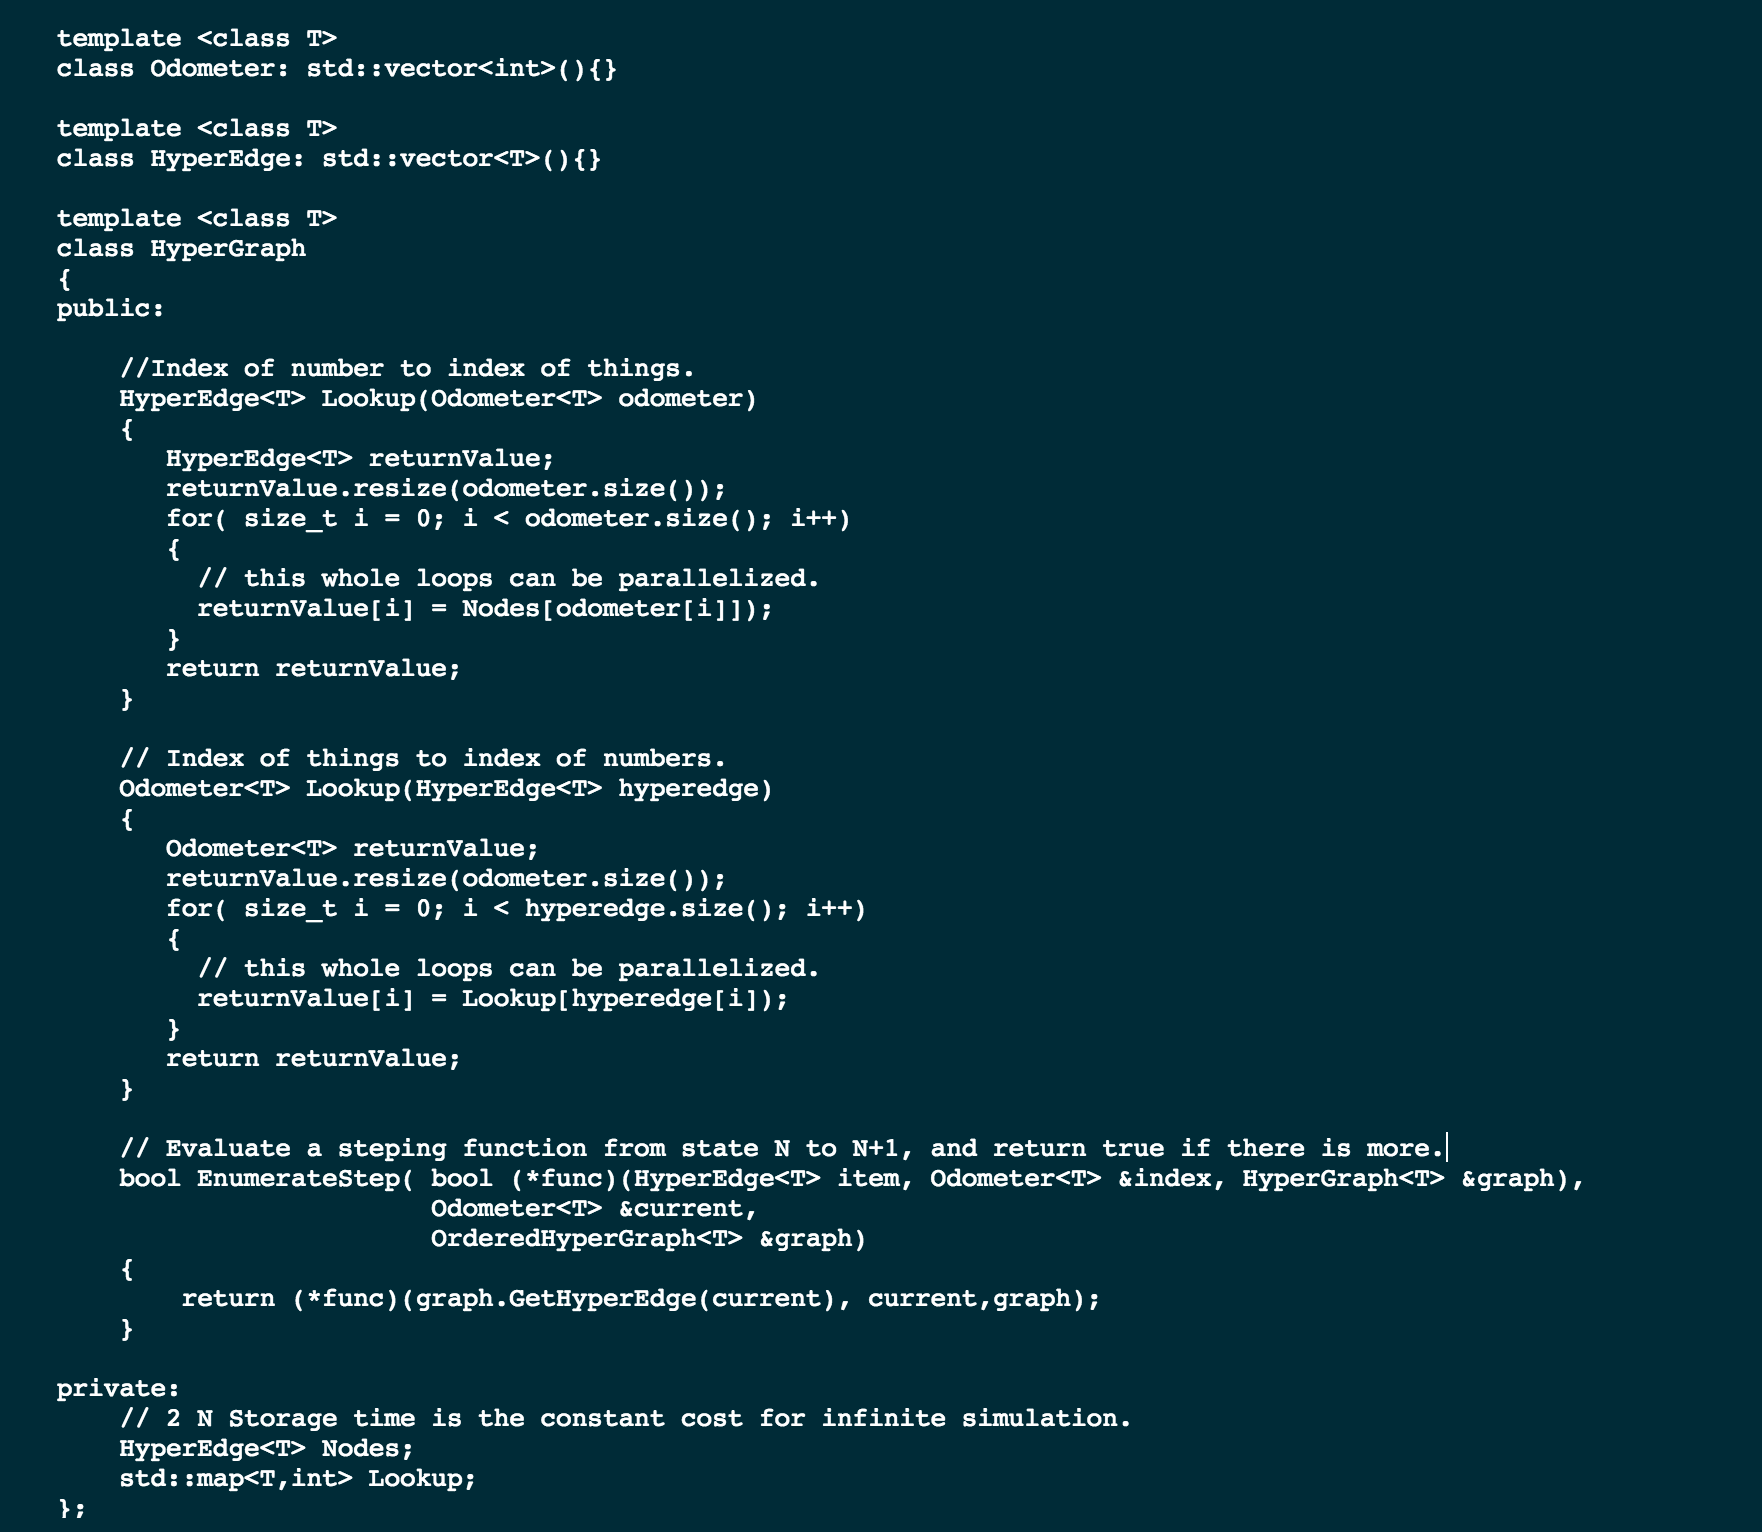
\includegraphics[width=10.75cm, height=8.5cm]{HypergraphCodeListing}
	\end{frame}	
	
	\begin{frame}
	\frametitle{Directed vs. undirected vs. ordered}
	\begin{itemize}
	\item Terminology for lists \{push,pop,indexof\} is not used for tree operations.
	\item Nomenclature from trees \{Child, Sibling, Parent, ect\} is not used in graphs.
	\item Directed and Undirected terminology originates from graphs
	\item Hypergraphs inherently rely upon indexes of numbers to access hyperedges/odometers.
	\item The odometer ordering determines the hyperedge ordering.
	\item The hyperedge ordering determines the odometer ordering.
	\end{itemize}
	\end{frame}
	
	\begin{frame}
	\frametitle{Ordered hypergraphs}
	\begin{itemize}
	\item Terminology for lists \{push,pop,indexof\} is not used for tree operations.
	\item Nomenclature from trees \{child, sibling, parent, ect\} is not used in graphs.
	\item Directed and undirected terminology originates from graphs
	\item Hypergraphs inherently rely upon indexes of numbers to access hyperedges/odometers.
	\item The odometer ordering determines the hyperedge ordering.
	\item The hyperedge ordering determines the odometer ordering.
	\end{itemize}
	\end{frame}
	
	\begin{frame}
	\frametitle{Ordered hyperedges}
	\begin{itemize}
	\item Permutations can be reduced to vombinations.
	\item Hyper-edges can be explored via adding additional nodes to them and translating back to odometer.
	\item Odometers can be explored via adding / subtracing numbers and translating them back to hyperedges.
	\item Modulo memory space turns indexing past the end into repeated data.
	\item Rounded memory space turn negative index into repeated data. 
	\end{itemize}
	\end{frame}
	
	
	\begin{frame}
	\frametitle{Converting odometers \& hyperedges given a hypergraph}
    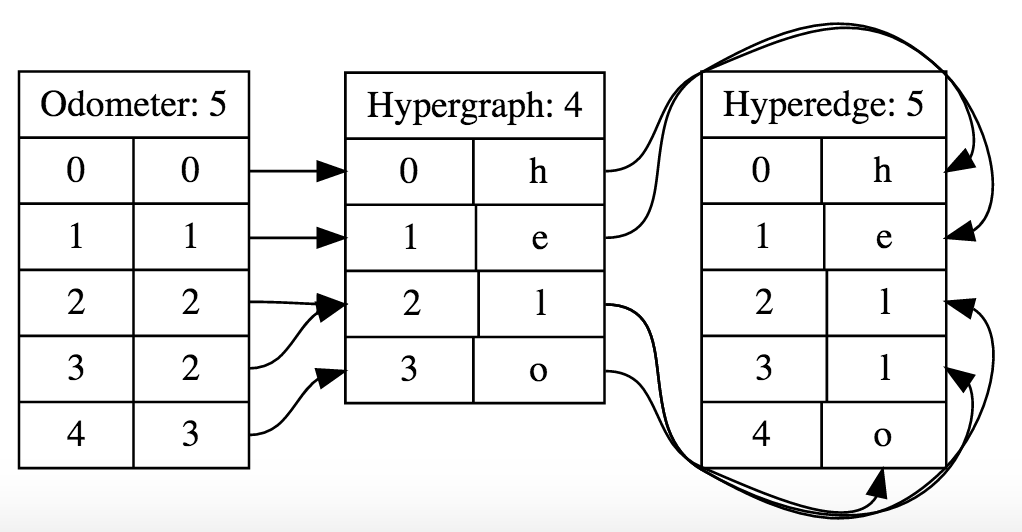
\includegraphics[width=8cm, height=3.75cm]{HelloHyper} \\
	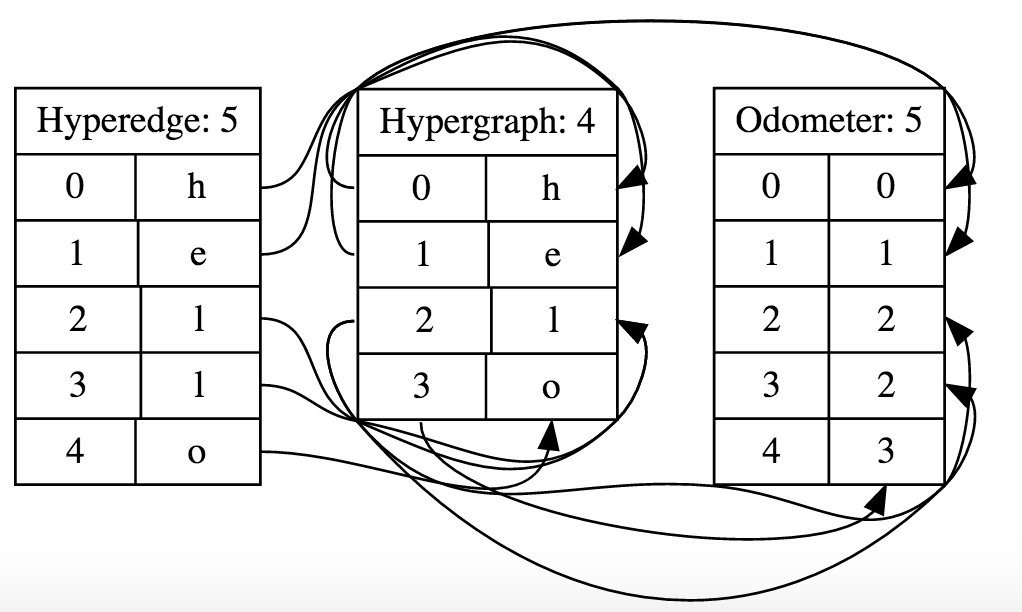
\includegraphics[width=8cm, height=3.75cm]{HelloOdometer}
	\end{frame}	
	
	\begin{frame}
	\frametitle{Explicit control of odometer determines next state to visit}
	\begin{itemize}
	\item Enumerating all hyperedges whose odometer size is 2 is equivelent to a fully connected graph.
	\item Accessing each hyperedge is constant time in the size/count of the odometer/hyperedge $O(c)$.
	\item As there are an infinite number of edges, we cannot visit them all as $O(\infty * c) \rightarrow O(\infty)$
	\item Only guranteed to terminate functions are provided.
	\item Enumeration of hyperedges \& odometers is now the programmers responsibility. 
	\item Similar to std::begin() and std::end() for loop control... 
	\item Except the function only returns true/false as to if execution has completed. And the programmer needs to write it.
	\end{itemize}
	\end{frame}
	
	\begin{frame}
	\frametitle{Explicit odometer control}
	\begin{itemize}
	\item Control over the odometer / number stack allows the transition from *ANY* hyperedge to *ANY* hyperedge in one step. 
	\item Depth first, Breadth first search are trivial counter incrementers.
	\item Enumerating combinations, permutations, and multi-select-variants is a trivial task.
	\item Controling of depth and breadth / bound and branch is possible via external heuristics.
	\item Exploring the depth and breadth from a given set of nodes is a simple as converting to hyperedge, then to odometer and exploring numerically instead of quantitatively. 
	\end{itemize}
	\end{frame}
	
\end{document}
